% !TEX TS?program = pdflatexmk
\documentclass[a4paper, 12pt]{article}
\usepackage[english]{babel}
\usepackage[utf8]{inputenc}
\usepackage[utf8]{inputenc}


%\renewcommand{\baselinestretch}{1.0} 
                    
                    
%Margins
\usepackage[left=25.4mm, right = 25.4mm, top=25.4mm, bottom=25.4mm, includefoot]{geometry}
%geometry{a4paper, total={170mm,257mm}, left=25.4mm, right = 25.4mm, top=25.4mm, bottom=25.4mm}
\setlength{\parindent}{0in}
\usepackage{enumitem}
       
                   
%Adding Pictures
\usepackage{graphicx}
\usepackage{float}
          
                    
%Header and Footers
\usepackage{fancyhdr}
\pagestyle{fancy}
%\fancyhead{}
\fancyfoot{}
\fancyfoot[R]{ \thepage\ }
\renewcommand{\headrulewidth}{0pt} %change the pt width to insert header line
\renewcommand{\footrulewidth}{0pt} %change the pt width to insert footer line
\usepackage{amsmath}
\fancyhf{}
               
                    
%\rhead{\leftmark}
%\lhead{Guides and tutorials}
\rfoot{Centre for Civil Society \hspace{1mm} \textbar \hspace{1mm} www.ccs.in \hspace{2mm}  \thepage}
%\lfoot{\leftmark}% get the section heading on the footer 
            
                                      
%Tables
\usepackage{booktabs}
\usepackage{subfig}
\captionsetup{aboveskip=14pt,}
\captionsetup[table]{justification = centering}
	
                    
%Coloured Boxes
\usepackage{xcolor}
\usepackage{mdframed}
           
                    
%Custom Spacing
\usepackage{setspace}
         
                    
%Defining Colours
\definecolor{CCSbrown}{RGB}{163, 86, 37}
\definecolor{CCSgrey}{RGB}{105, 105, 105}
\definecolor{CCSblack}{RGB}{64, 64, 65} 
             
             
%Heading Colours                  
\usepackage{sectsty}
\usepackage{titlesec}
\chapterfont{\color{blue}}  %sets colour of chapters font
\sectionfont{\color{CCSbrown}}  %sets colour of section font
\subsectionfont{\color{CCSblack}} %sets colour of subsection font
\subsubsectionfont{\color{CCSblack}} %sets colour of subsubsection font
		
    				
%Bibliography
\usepackage[authordate, backend=biber]{biblatex-chicago}
\addbibresource{EWaste.bib}
\usepackage{hyperref} %activates links 
\hypersetup{
colorlinks,
linkcolor = black,
citecolor = CCSbrown,
urlcolor = black}
\usepackage{blindtext}
		
              
\begin{document}
                    
%==================================================                

%Title Page
\begin{titlepage}
\begin{center}
\line(1,0){300}\\
[0.25in]
\huge{\bfseries\textcolor{CCSbrown} {Toxic Efficiency}} \\
[0.5cm]
\large{Refining Extended Producer Responsibility \\ for E-Waste in India} \\
    	
\line(1,0){200}\\
[1in]
\textsc{\huge Tarini Sudhakar, Akshat Singh, \\ Shubham Singh} \\
[1.5cm]
{\Large September 2018} \\
[2.0cm]

{\LARGE Centre for Civil Society} \\
[0.1mm]
{\Large New Delhi, India} \\
[2.0cm]

\includegraphics[width = 75mm]{CCSlogo.jpg}
      
\end{center}
\end{titlepage}

%=====================TOC============================                 
                    \tableofcontents
                    
%======================LIST OF ABBREVIATIONS==========       
\newpage
\newlist{abbrv}{itemize}{1}
\setlist[abbrv,1]{label=,labelwidth=1in,align=parleft,itemsep=0.1\baselineskip,leftmargin=!}

%List of Abbreviations         
\section*{List of Abbreviations}
\addcontentsline{toc}{section}{List of Abbreviations}
        
\begin{abbrv}
         
        \item[CPCB]			Central Pollution Control Board
        \item[CTE]				Consent to Establish
        \item[CTO]			Consent to Operate
        \item[DIC]				District Industries Centre
        \item[DRS]			Deposit Refund Scheme
        \item[EEE]				Electronics and Electrical Equipment 
        \item[EPR]				Extended Producer Responsibility
        \item[ETP]				Effluent Treatment Plant 
        \item[GoI]				Government of India
        \item[EWM]			E-Waste Management
        \item[HWM]			Hazardous Waste Management
        \item[MoEFCC]			Ministry of Environment, Forest and Climate Change
        \item[IT]				Information Technology 
        \item[MTA]				Metric Tonnes per Annum
        \item[NCR]			National Capital Region
        \item[PET]				Polyethylene Terephthalate
        \item[PRO]			Producer Responsibility Organisation
        \item[SPCB]			State Pollution Control Board
        \item[TSDF]			Treatment, Storage and Disposal Facility
        \item[UP]				Uttar Pradesh
        
        
         
\end{abbrv}
        
                    
%Executive Summary
\newpage
\section*{Executive Summary}
\addcontentsline{toc}{section}{Executive Summary}
                    
                    India generates two million metric tonnes of e-waste annually and ranks amongst the top five e-waste generating countries in the world \parencite{shenoynews}. The informal sector handles almost 95\% of this amount through the process of dismantling or refurbishing \parencite{assochamstats}. Only 5\% of the total e-waste is recycled, and 90\% of this is recycled informally \parencite{assochamstats, kumarnews}. The authorised recycling sector in India is still nascent while informal recycling operations have been in place for a long time, employing over one million people \parencite{baldereport}. \\
                    
                    The profit inherent to recycling e-waste lies in extracting and selling metals from electronic products. While it is profitable to extract metals like gold and copper, the extraction of toxic substances, such as mercury and lead, is not as financially rewarding \parencite{worstallnews}. Moreover, these hazardous substances need to be disposed of properly. \\
                    
                    Unfortunately, informal recyclers circumvent the cost of treating these toxic components by dumping them in the open. This neglect contaminates the soil and pollutes water bodies. \\
                    
                    The Government of India (GoI) has attempted to divert the flow of e-waste from the informal sector to the formal sector through the Extended Producer Responsibility (EPR) model introduced in the E-Waste Management (EWM) Rules, 2011. Producers—defined in the EWM Rules, 2011 as any people who manufacture or sell electrical and electronic equipment and their components—are obligated under EPR to channelise the e-waste generated by their products to authorised recyclers. They do so by collecting their products back from the consumers and selling the e-waste to the authorised recyclers. \\
                    
                    However, this envisioned EPR model does not match the actual flow of e-waste in India. Interviews with authorised recyclers in India showed that many of the 178 authorised recycling firms registered with the Central Pollution Control Board (CPCB) in 2016 are currently performing under-capacity or running at a loss while the informal sector controls a significant portion of the e-waste market. Our survey revealed that this is because informal recyclers quote at least double the prices offered by the authorised recyclers for buying e-waste. Through this study, we attempt to understand the factors that hinder the authorised recycling sector from competing with the informal sector. \\

                    The \hyperref[sec:1]{first section} of the paper examines the EPR model in India and the changes brought forth by the EWM Rules, 2016, to check the leakages to the informal sector. These adjustments include the introduction of mandatory collection targets and collection mechanisms other than take-back schemes and collection centres. \\
                    
                   The \hyperref[sec:2]{second section} compares the intended flow of e-waste with its actual movement and claims that despite revising the 2011 Rules, authorised recyclers are unable to thrive in comparison to informal recyclers. Our survey of six recycling firms in Faridabad, Rohtak, Manesar and Hapur showed that these authorised recyclers were operating at 39.9\% of their total capacity to recycle e-waste. \\
                   
                   The \hyperref[sec:3]{third section} explores the possible reasons for this dissonance and the failure of the current EPR model. We argue that the current model fails to accommodate the higher prices offered by the informal recycler to buy e-waste. For instance, an HP laptop sells for Rs. 4,642.9 in the informal sector compared to Rs. 1,133.3 in the authorised.\\
                   
                   We hypothesise that the price difference between authorised and informal recyclers is the result of the latter’s operational efficiency \parencite{chintanreport}. Using this as a base, we study the operating costs for both authorised and informal recyclers. These include the licences required to enter the authorised recycling market, compliance with government regulations, secure disposal of hazardous residue, and secondary markets for refurbished goods. These costs could keep authorised recyclers from quoting prices similar to those of informal recyclers who operate without the necessary licences. For instance, the average official time taken to obtain Consent to Establish and Consent to Operate from the Haryana and Uttar Pradesh State Pollution Control Boards (SPCBs) for recycling e-waste is 1.3 months. According to our survey, the actual time taken to acquire these licences ranges from less than 1 month to 24 months. Therefore, the actual time taken to obtain licences could serve as a transaction cost for authorised recyclers.\\
                    
                    The \hyperref[sec:4]{last section} lays out a proposal for a revitalised EPR model that tackles the price difference between authorised and informal recyclers in India. Our model suggests three modifications to the existing EPR system in the form of a mandatory Deposit Refund Scheme (DRS), a Common Deposit Account, and third-party audits.\\
                    
                     First, the mandatory DRS incentivises the consumers to return their devices to the producers and not the \textit{kabadiwala}.\footnote{A \textit{kabadiwala} is a small-scale scrap collector who regularly purchases unwanted items such as newspapers, mobile phones and old television sets, from households.} DRSs have been shown to increase recycling rates. After the implementation of a mandatory DRS, the recycling rate for lead-acid batteries in the USA rose from 86\% to 97\% \parencite{wallspaper}. Second, the Common Deposit Account enhances the efficiency of our model. It collects all the Deposit Refund fees into a common account, which allows the consumers to return their devices to any producer. Finally, the third-party audits check e-waste from moving to the informal sector.\\
                    
%Introduction
\newpage
\section{Introduction}
                    
                    The production of electronic appliances has been steadily rising over the years, and there are no signs of their demand waning anytime soon \parencite{chidambarampaper}. The electronics and hardware industry of India is expected to grow at a compound annual growth rate of 12\% to 13\% and reach \$112 to \$133 hundred crores by 2018 \parencite{assochameyreport}. New producers from Brazil, India and China and the widespread use of semiconductors have been instrumental in bringing down the cost of manufacturing electronic devices and hence, their prices \parencite{ahmednews}. \\
                    
                    The fall in prices alongside a growing middle class with an increasing disposable income contributes to a larger market for electronics and electrical equipment (EEE) \parencite{assochamnecreport}. Consumers are driven to replace functional products as soon as newer models enter the market. Planned obsolescence may have also increased the units of EEE sold to replace products from 3.5\% in 2004 to 8.3\% in 2012 \parencite{alanews}. \\
                   
                   This rise in the manufacture of EEE has been simultaneously followed by an increase in the amount of e-waste or end-of-life EEE generated. The global volume of e-waste is expected to reach 52.2 million metric tonnes per annum (MTA) by 2021 at an annual growth rate of 3.15\% \parencite{assochamstats}. \\ 
                    
                    E-Waste is a pertinent ecological issue. EEE include certain components that are made of valuable metals such as gold and copper. It is profitable to process these parts and sell the metals as raw material. However, electronic products also contain a mix of toxic elements like mercury and lead. These hazardous constituents are often not recycled because it is deemed more economical to recycle the valuable metals and dispose of the rest \parencite{worstallnews}. If disposed of improperly, these toxic components can cause significant environmental damage by contaminating the topsoil and leaching into the groundwater. \\
                    
                    Government interventions are necessary to encourage and facilitate the safe disposal of hazardous residue. Accordingly, the Government of India (GoI) has issued the E-Waste Management (EWM) Rules, 2016. As per these rules, e-waste management in India is under the ambit of the Ministry of Environment, Forest and Climate Change (MoEFCC). The MoEFCC has mandated producers and recyclers to obtain ‘authorisation’ under the EWM Rules, 2016, and Hazardous and Other Wastes (Management and Transboundary Movement) (HWM) Rules, 2016.\footnote{Only applicable to those who process e-waste that comes under Part C, Schedule III of the HWM Rules, 2016.} Producers and recyclers are allowed to continue operations in India only if they meet necessary standards for the safe and proper handling of e-waste. \\
                     
                     Despite these regulations, more than 95\% of the generated e-waste ends up with the informal sector, which operates without the necessary authorisations \parencite{assochamstats}. Much of the informal recycling takes place through open burning, grinding and washing, and acid baths \parencite{csereport}. These processes are highly dangerous and release toxic elements into the environment. For instance, informal recyclers dump high amounts of ash left over from burning e-waste in the Ramganga River in Moradabad, Uttar Pradesh (UP) \parencite{csereport}. \\
                    
                    Informal recyclers further amplify the problem by dumping the non-recycled hazardous components openly on the riverside or the ground. Studies show that the soil in areas such as Loni, Mandoli and Krishna Vihar in New Delhi is deeply contaminated with heavy metals \parencite{toxicsreport, sahanews}. Moreover, informal workers also do not have the necessary tools for the safe handling and recycling of e-waste \parencite{kumarnews}. This neglect leads to severe (individual and public) health repercussions \parencite{bhowmicknews}. \\
                    
                    In order to divert the supply of e-waste to the authorised sector, the GoI introduced the concept of EPR to e-waste in India in 2011. The concept was adopted after it successfully solved similar problems in other countries. However, its implementation in India has not delivered the expected results. The informal sector still processes most of the e-waste in India while authorised recyclers struggle to operate competitively. \\
                    
                    In this paper, we look at the current design of EPR in India, examine its shortcomings and propose improvements to cover its limitations. Our study is based on interviews with authorised and informal recyclers operating in the National Capital Region (NCR) of India.  
                    
%Extended Producer Responsibility for E-Waste in India
\section{Extended Producer Responsibility for E-Waste in India}\label{sec:1}
                    
                    On 8 April 2010, a man was exposed to Cobalt 60 while attempting to dismantle radioactive pipes in Mayapuri—one of the informal e-recycling hubs in Delhi. He died 19 days later due to the adverse effects of the radiation. There were several other victims of the same \parencite{bhadurinews}. The outcry that followed pushed the government into passing the EWM Rules in 2011. \\
                    
                    While many environmental regulations were put in place in India for managing hazardous waste, until 2011, e-waste was only dealt with briefly under two laws—the Hazardous Waste Management (HWM) Rules, 2008, and the Batteries (Management and Handling) Rules, 2001. The government had not enacted any rules that were explicitly dedicated to e-waste. This patchwork of legislation was hampered without an effective enforcement of the existing regulations \parencite{kumarsinghpaper}. For instance, the HWM Rules, 2008, required any person recycling or reprocessing hazardous waste, including e-waste, to acquire authorisation from the CPCB. However, only 23 recyclers had been authorised under the HWM Rules until 2010 \parencite{bhaskarturagapapera}. \\
                    
                    The informal sector predominantly handled the supply of e-waste \parencite{thakurnews}. The consumer would sell EEE products to their local \textit{kabadiwala}. The \textit{kabadiwala} then resold the collected waste to the local scrap dealers. The scrap dealers sorted the waste and sold it to the informal dismantlers, refurbishers and recyclers. \\
                    
                    The EWM Rules, 2011, defined electronic waste or e-waste as ‘electrical and electronic equipment that has been discarded in whole or in part by individual and bulk consumers and during manufacturing, refurbishment and repairing processes’ and introduced the concept of EPR. 

%Concept of Extended Producer Responsibility                     
\subsection{Concept of Extended Producer Responsibility}
                    
                    EPR holds the producer physically or financially responsible for the total environmental damage caused by his/her product at the end of its lifespan \parencite{wallschapter}. Thomas Lindhqvist, a Swedish academic, introduced the concept of EPR to the Government of the Kingdom of Sweden in 1990. It was then implemented for the first time in 1991 in Germany to manage the waste generated by the packaging industry \parencite{toxicspaper}. \\
                    
                    When EPR is implemented in a sector, the producer’s responsibility is extended from the product’s manufacturing and consumption to its treatment at the end of its life \parencite{toxicspaper}. For example, consider the implementation of EPR in the bottled water sector. In a world without EPR, a company selling bottled water in polyethylene terephthalate (PET) bottles would only be responsible for the quality of the bottle and the water within. Despite the pollution risk posed by the PET bottles, neither the company nor the consumer would be liable for its safe disposal. With EPR, the company would be responsible not only for the water and its packaging but also for ensuring the secure disposal of the PET bottles after usage. \\
                    
                    In traditional waste management models, consumers bear the burden of ensuring proper waste disposal. The local administration taxes consumers, and the revenue generated is used to run a waste management system. Since producers have no incentive to reduce the negative environmental externalities caused by their products, there is no change in the volume of e-waste generated, toxicity or the safe disposal of EEE components. EPR changes the incentive structure and holds the producers responsible for the inflicted environmental harm \parencite{bhaskarturagapaperb}. 

%Current Design of Extended Producer Responsibility for E-Waste in India                    
\subsection{Current Design of Extended Producer Responsibility for E-Waste in India}
                    
                    With the objective to ensure the safe disposal of e-waste, the EWM Rules, 2011, brought EPR to waste management in India, making producers \footnote{Defined in the EWM Rules, 2011, as 'any person who manufactures or sells electrical and electronic equipment and their components'.} of EEE responsible for collecting their e-waste and treating it appropriately. \\
                    
                    However, the rules failed to achieve the anticipated results. While registered recycling capacities increased, authorised recyclers still received only 5\% to 15\% of the total supply of e-waste \parencite{bhaskarturagapapera}. Instead of encouraging the development of better collection and recycling infrastructure, the EWM Rules, 2011, ended up compelling the producers to implement a few inexpensive aspects of EPR \parencite{bhaskarturagapapera}. \\
                    
                    The EWM Rules, 2016, were implemented to fix these shortcomings.\footnote{After issuing the EWM Rules, 2011, the GoI released the EWM Rules, 2016. This set of Rules was amended in March 2018 and came to be known as the EWM Amendment Rules, 2018.} Three major changes that came under the new rules were modifications to the EPR Authorisation process, addition of various collection mechanisms for the producers to comply with EPR, and institution of mandatory collection targets. If the producers defaulted on any of these counts, they could be charged financial penalties approved by the CPCB under the Environmental Protection Act, 1986.\footnote{See Rule 21 (2) of the EWM Amendment Rules, 2018.}

%Extended Producer Responsibility Authorisation                    
\subsubsection{Extended Producer Responsibility Authorisation}
                    
                    Granted by the CPCB under the EWM Rules, 2016, EPR Authorisation ensures that producers can be held accountable for channelling their e-waste to authorised recyclers. The authorisation requires a detailed EPR Plan outlining the mechanism chosen by producers for EPR implementation and agreements with authorised dismantlers and recyclers. It also helps the government maintain a record of all the firms processing e-waste in the country. As per Rule 13 (1) (iv) of the EWM Rules, 2016, if the producers’ applications for EPR Authorisation fail, their operations will be stopped until they are duly authorised to exercise EPR. 
                 
%Collection Mechanisms                         
\subsubsection{Collection Mechanisms}
                    
                    EWM Rules, 2011, had failed to mention any specific method apart from setting up collection centres and instituting take-back arrangements for implementing EPR. This ambiguity contributed to the difficulty of its execution \parencite{pibreport}. For example, a study undertaken in 2015 showed that almost 35\% of the major EEE (both international and domestic) producers in India had either taken zero or limited action to implement EPR. Another 29\% had attempted to set up mechanisms but failed to achieve positive results. Most of these producers neither established take-back systems nor conveyed information about e-waste to their consumers, as directed in the EWM Rules, 2011 \parencite{toxicsreportb}. \\
                    
                    Therefore, to make it easier for the producers to implement their EPR, EWM Rules, 2016, offered new instruments for channelising the e-waste towards authorised recycling and disposal. These included the DRS and Producer Responsibility Organisations (PROs).
                    
%Collection Centres                    
\paragraph{Collection Centres} 
                    
                    According to the EWM Rules, 2011, collection centres—points or centres set up to gather e-waste—had to acquire authorisation from the State Pollution Control Boards (SPCBs) to operate. The EWM Rules, 2016, removed the need for this authorisation to allow flexibility for the producers while executing their EPR (PIB 2016). They could now be set up by an individual producer or an association, PROs, dismantlers or recyclers in order to channel waste to the authorised recyclers \parencite{pibreport}. 
                    
%Deposit Refund Scheme
\paragraph{Deposit Refund Scheme}
                    
                    Under the EWM Rules, 2016, producers who implement a DRS charge an additional amount as a deposit at the time of sale of EEE. Consumers receive this amount (along with the appropriate interest) only when they deposit the EEE at the end of its life with producers. In this manner, the deposit incentivises consumers to return used products to producers. 
                    
%Producer Responsibility Organisation
\paragraph{Producer Responsibility Organisation}
                    
                    PROs serve as a means for producers to outsource their EPR implementation to meet collection targets. PROs aid producers by setting up and running collection centres and spreading awareness about e-waste to consumers. They can also enact mechanisms such as a take-back or a DRS \parencite{cpcbproreport}. \\
                    
                    The EWM Rules, 2016, recognise the PROs as an important stakeholder in the e-waste market in India. Given their steadily growing presence, PROs are now required to register with the CPCB as per Rule 13 (1) (xvii) of the EWM Amendment Rules, 2018. Upon failure to do so, the PROs would face penalisation under the Environmental Protection Act, 1986.\footnote{See Guideline 11 in Guidelines for Producer Responsibility Organization (PRO), CPCB.} 
                    
%Mandatory Collection Targets 
\subsubsection{Mandatory Collection Targets}
                    
                    The EWM Rules, 2016, also sought to improve the success rate of EPR implementation by introducing mandatory minimum collection targets for each producer (PIB 2016). The EPR collection target was set as 30\% of the quantity of waste generated by the producers for 2016 to 2018.\footnote{See Schedule III of the EWM Rules, 2016} This target would increase in subsequent years, and by 2022, the producers would have to collect 70\% of the waste generated. \\
                    
                    However, in March 2018, the MoEFCC amended the EWM Rules, 2016, and reduced the collection targets. Producers were required to collect only 10\% of the e-waste generated in 2017 to 2018 with 10\% annual increments. After 2022, they would need to meet the EWM Rules target of 70\% waste generated.\footnote{See Schedule III of the EWM Amendment Rules, 2018.} This mandated rate is significantly higher than the collection rates in many developed countries, which plateau between 40\% and 50\%. Nonetheless, it should be noted that consumers in these countries bear the cost of recycling unlike in India, where recyclers pay them for e-waste \parencite{veitreport}. \\
                    
                    The amendment also introduced separate EPR targets for newer producers.\footnote{See Schedule III A of the EWM Amendment Rules, 2018.} As per Rule 13 (1) (xii) in the EWM Amendment Rules, 2018, these new producers were defined as those who had been operating in the market for a shorter period than their product’s average lifespan. Their EPR collection targets were based on the previous year’s sales figures and were lower than the targets for the older producers.\footnote{\textit{Ibid.}}                      
                    
%Movement of E-Waste after Extended Producer Responsibility
\section{Movement of E-Waste after Extended Producer Responsibility}\label{sec:2}
                    
                    The EWM Rules, 2016, made important changes to the EPR model in order to divert the supply of e-waste to the authorised recyclers. However, the actual movement of e-waste continues to differ significantly from the intended direction, as the informal sector still handles more than 95\% of the domestically generated e-waste \parencite{assochamstats} while authorised recyclers are unable to engage a competitive portion of the market.

%Intended Flow of E-Waste                                  
\subsection{Intended Flow of E-Waste}
                    
                    The mechanism envisioned in the EWM Rules, 2016 (see Figure 1) to reroute the flow of e-waste to the authorised recyclers involved four key steps.                     
\begin{enumerate}
\item After using the EEE, the consumers would deposit the product (e-waste) with the authorised producers.
\item Mandated targets would compel producers to collect the e-waste by employing one (or a combination) of the several collection mechanisms. 
\item The producers would channel the collected e-waste to authorised recyclers.
\item The recyclers would then choose to either recycle or refurbish the e-waste and send the hazardous residue to Treatment, Storage and Disposal Facilities (TSDFs).
\end{enumerate}
                    
                    The government would place two checks to ensure that the objective of EPR is fulfilled. First, it would monitor the producers to ensure that they meet the annual collection targets.\footnote{As per Rule 5 (4) of the EWM Rules, 2016, producers are required to submit an annual report detailing the e-waste handled.} Second, it would audit the authorised recyclers to ensure that they dispose of hazardous material safely.\footnote{As per Rule 11 (8) of the EWM Rules, 2016, recyclers are required to submit an annual report detailing the e-waste collected, dismantled and recycled.}\\
                    
%Figure 1
\begin{figure}[H] %H means Here (HTPB = Here, Top, Page of Float, Bottom)
\centering
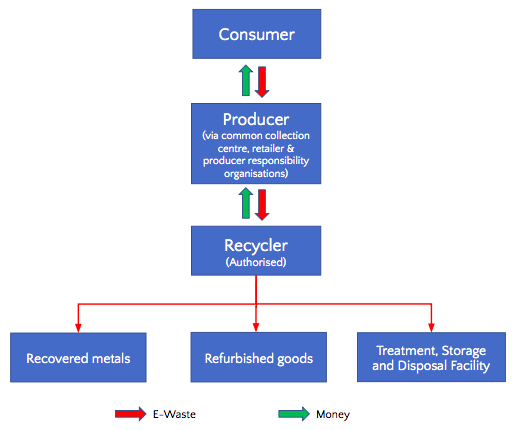
\includegraphics[height = 4.3in]{fig1.png}
\caption[Optional Caption]{The EPR Model in India as per the EWM Rules, 2016}
\end{figure}
                    
%Actual Flow of E-Waste
\subsection{Actual Flow of E-Waste}
                    
                    In reality, the flow of e-waste in India is much more complicated. Based on our interaction with authorised and informal recyclers, we realised that the EPR model visualised in the EWM Rules, 2016, was not functioning as intended.\\ 
                    
                    For instance, the NCR generates 85,000 metric tonnes of e-waste annually and has 28 recycling firms with a capacity of 1,07,976 MTA \parencite{assochamdelhi, cpcbrecyclersreport}. However, our survey of six recycling firms in Faridabad, Rohtak, Manesar and Hapur showed that these authorised recyclers were operating at 39.9\% of their total capacity (see Appendix 1). Their capacity to process e-waste was far greater than the amount they were recycling. \\
                    
                    Instead, most of the e-waste is being diverted to the informal recyclers in the following manner.                    
\begin{enumerate}
\item After using the EEE, the individual consumers sell the product (e-waste) to the \textit{kabadiwala} instead of the authorised collection entities. The \textit{kabadiwala} resells the waste to the informal recycler who processes it unsafely. 
\item The authorised producers meet their mandated targets by collecting their e-waste from bulk consumers like information technology (IT) companies. It is more economical to meet a 10\% collection target by focusing on the bulk consumers than implementing any of the collection mechanisms specified in the EWM Rules, 2016.
\item Producers sell this e-waste to authorised recyclers. However, authorised recyclers do not process the e-waste.  
\item Instead, the authorised recycler sells the e-waste to the informal recyclers. These informal recyclers, after processing the waste, continue to dump the hazardous residue improperly.
\end{enumerate}
                    
                    The checks placed by the government have proven to be ineffective. In our interviews with the formal recyclers, we noted that some authorised producers and recyclers sold the e-waste that they had collected to the informal recyclers. \\
                    
                    Our visit to Seelampur corroborated this circumvention of regulations. We posed as potential consumers looking to sell e-waste and asked if we could have some legitimate proof of our transaction. In response, the informal recycler offered us a certificate that verified his status as an authorised recycler and a Goods and Services Tax transaction ID validating our sale. He bought these documents from other authorised recyclers for a certain fee. If we chose to take the documents verifying our transaction, he would accommodate this fee in the e-waste prices quoted to us. In this manner, the formal sector diverted e-waste towards the informal recyclers. \\
                    
                    We argue that in reality, e-waste in India moves along the channels shown in Figure 2. \\
                    
%Figure 2
\begin{figure}[H]
\centering
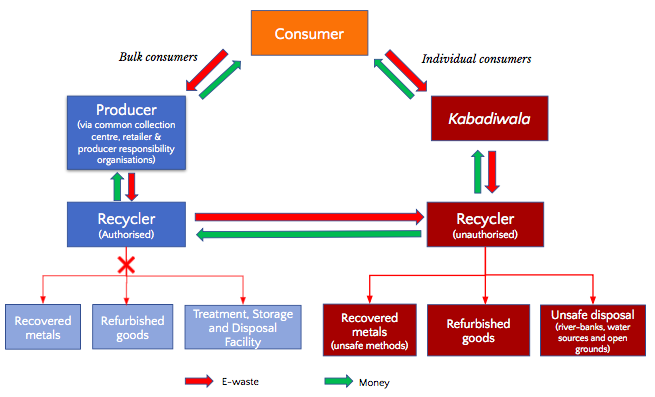
\includegraphics[height = 4in]{fig2.png}
\caption[Optional Caption]{Actual Flow of E-Waste in India}
\end{figure}
                    
%Price Difference Between Authorised and Informal Recyclers
\section{Price Difference Between Authorised and Informal Recyclers}\label{sec:3}
                    
                    To understand why consumers were routing e-waste to informal recyclers, we visited some of the e-waste hubs of Delhi—namely, Seelampur and Shastri Park.\\
                     
                     In 2013, the Chintan Environmental Research and Action Group evaluated the prices offered by both informal and authorised recyclers in Shastri Park, Seelampur and Turkman Gate \parencite{chintanreport}. Using this study as a base, we averaged the prices offered for end-of-life EEE by seven informal shops in Shastri Park and Seelampur and five authorised recycling firms spread across the NCR (Faridabad, Hapur and Panipat).\\
                     
                     Informal recyclers quoted at least double the prices offered by authorised recyclers (see Appendix 2). ACs and computer monitors were exceptions; the prices given by both were similar.\footnote{The reason for the similarity in prices for these products has not been examined in this paper.} However, this price difference (see Figure 3) allowed the informal recyclers to attract more e-waste than the authorised recyclers. \\
                                        
%Figure 3
\begin{figure}[H]
\flushleft
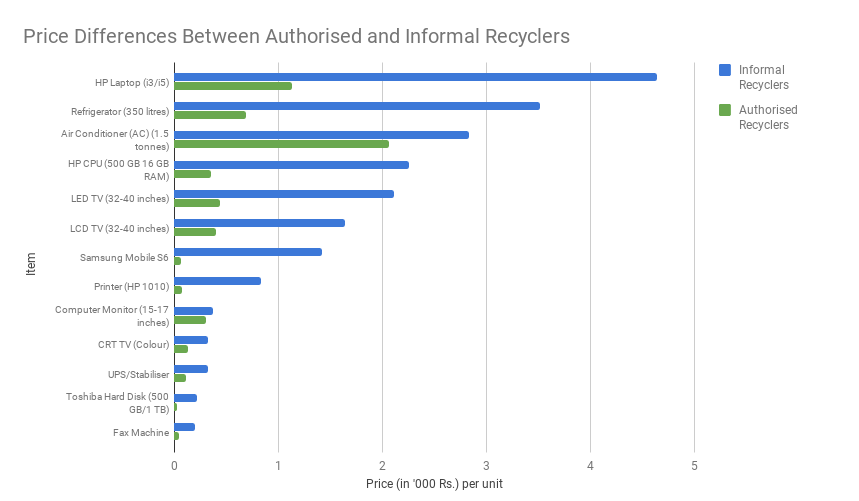
\includegraphics[height= 4.20in]{fig3.png}
\caption[Optional Caption]{Visualisation of Price Difference Between Authorised and Informal Recyclers}
\end{figure}
                    
%Understanding Operational Efficiency
\subsection{Understanding Operational Efficiency}
                    
                    Informal recyclers function with far lower operating costs than authorised recyclers in India do. These costs allow them to quote higher prices and capture a significant portion of the market \parencite{chintanreport}. In this section, we offer explanations accounting for the price difference between authorised and informal recyclers. 
                    
%Cost of Licences
\subsubsection{Cost of Licences}
                    
                    Under the EWM Rules, 2016, a recycler needs to acquire certain licences to begin operations. We hypothesised that the cost of acquiring these licences was significant and would ultimately reflect in the price that the authorised recyclers could afford to pay for the e-waste. Informal recyclers do not bear this cost, as they operate without the necessary licences. \\
                    
                    An authorised recycler needs to acquire the following registrations/licences to start processing e-waste:                  
\begin{enumerate}
\item \textit{Consent to Establish} (CTE) from the SPCB;
\item \textit{Consent to Operate} (CTO) from the SPCB;
\item \textit{Certificate of Registration} from the District Industries Centre (DIC);
\item \textit{Proof of Installed Capacity} of plant and machinery from the DIC;
\item \textit{Environmental Clearance} from the SPCB; 
\item \textit{E-Waste Licence} under the EWM Rules, 2016 from the SPCB;
\item \textit{Hazardous Waste Licence} under the HWM Rules, 2016 from the SPCB.\footnote{For firms which handle waste that comes under Part C, Schedule III of the HWM Rules, 2016.} 
\end{enumerate}
                    
                    As the Environmental Clearance (No. 5) was required for plants with a capacity greater than 25,000 MTA and only 2 of the 178 registered plants had this capacity, its cost has been omitted from our calculations \parencite{cpcbrecyclersreport}. The cost of registering with the DIC (No. 3 and No. 4) is also not included due to logistical restraints.\\
                    
                    The official costs for the E-Waste Licence and Hazardous Waste Licence comprise the cost of acquiring standard industry licences—CTE and CTO (No. 1 and No. 2). The official costs for these licences vary according to the initial investment of the firm. Through our interviews, we gauged this initial investment for a recycling firm to be between Rs. 1 and 5 crores. We then computed the official costs levied by each SPCB for the industry licences using the information provided on the respective SPCB websites.\\ 
                    
                    As our study focuses on the NCR, we specifically looked at the costs imposed by UP and Haryana. We tried to capture the actual time taken to acquire the licences as it may have been a source of transaction costs. However, we were only able to survey six firms in the NCR. Therefore, we calculated the official time taken to grant licences in UP and Haryana. Table 1 records these costs. \\
          
%Table 1         
\begin{table}[htpb]
\caption{Official Cost of Acquiring CTE and CTO}
\begin{tabular}{ l  l  c  r } %Alignment of Text
\toprule
 \multicolumn{1}{p{7em}}{State} & \multicolumn{1}{p{7em}}{Licence} & \multicolumn{1}{p{11.5em}}{Cost in Rs. \centering\footnotesize\textit{(For Investment Between 1 and 10 crores)}} & \multicolumn{1}{p{8.75em}}{{Official Time Taken} \raggedleft\footnotesize\textit{(in days)}}\\ 

\midrule
Uttar Pradesh & CTE + CTO & 1,17,000 & 40-60\\
Haryana & CTE + CTO & 3,84,000 & 20-40\\
\bottomrule
\end{tabular}
\end{table}
                    
                    The official costs for these licences range between Rs. 1 and 4 lakhs. The average official time taken to obtain them is 1.3 months. According to our survey, the actual time taken to acquire these licences ranged from less than 1 month to 24 months.

%Cost of Regulatory Compliance                    
\subsubsection{Cost of Regulatory Compliance}
                    
                    Authorised recyclers need to comply with other regulations that the informal sector does not need to. Auditing and physical inspections are part of the scrutinisation process. These provisions place a check on the e-waste handled by producers and recyclers and impose an additional cost on them. Informal recyclers do not incur these costs nor do they pay the appropriate taxes levied on authorised recyclers. \\
                    
                    There are also costs associated with adhering to labour regulations. An authorised recycler needs to implement specific occupational and safety measures before starting operations (see Appendix 3). However, informal recyclers often work with the bare minimum gear and do not comply with these rules. They also do not abide by child labour laws as over 4.5 lakhs children are allegedly employed by the informal sector \parencite{assochamchild}.
                    
%Cost of Disposing Hazardous Residue 
\subsubsection{Cost of Disposing Hazardous Residue }
                    
                    Authorised recyclers incur additional costs when they attempt to meet the standards set by government regulations. However, even if these regulatory costs were lifted, authorised recyclers would still have to pay for safely disposing of the hazardous residue.\\
                     
                     The regulations in place to oversee the secure disposal of toxic components require authorised recyclers to send their processual residue to authorised TSDFs.\footnote{See Rule 11 (7) of the EWM Rules, 2016.} Informal recyclers circumvent this obligation and avoid the cost of treating their toxic waste in TSDFs by dumping it in the open.
                    
%Access to Secondary Markets for Refurbished Goods 
\subsubsection{Access to Secondary Markets for Refurbished Goods}
                    
                    An often-overlooked element of the e-waste market is the refurbishment and reuse of waste EEE. More than recycling, the informal recycler focuses on the reuse, resale and refurbishment of goods \parencite{gidwanicorwinpaper}. Much of e-waste is repaired and sold in secondary markets. These markets usually sell refurbished goods without obtaining prior approval from the producer companies. For example, in New Delhi, Nehru Place and Gaffar Market are prime secondary markets for EEE.\\
                    
                    Reselling refurbished goods is more profitable than merely selling recycled metal. Informal recyclers are at an advantage and can quote higher prices for the e-waste, as the authorised recyclers are often forbidden from reselling. The producer companies that employ authorised recyclers to handle their e-waste fear the creation of parallel competition for their new products \parencite{alevphd}. Our interviews with authorised recyclers revealed that some of their clients (producer companies) demanded that the recyclers photographed the shredded e-waste. This evidence ensured that the recyclers could not resell the waste EEE in the secondary markets.\\
                    
                    Numerous factors, such as the ones mentioned above, contribute to the price gap between authorised and informal recyclers. This price gap incentivises consumers to sell e-waste to the informal sector and thus, negates the envisioned EPR model.
 
                    
%Revitalised EPR Model
\section{Revitalised Extended Producer Responsibility \\ Model}\label{sec:4}
                    
                    In order to seal off the e-waste leakages to the informal market and make the authorised sector more competitive, the EPR model needs to tackle the difference in prices that authorised and informal recyclers offer to buy e-waste. We suggest three modifications to the current system: a mandatory DRS, a Common Deposit Account, and third-party audits. The mandatory DRS secures the supply of e-waste to the authorised recyclers, and audits are required to prevent e-waste from leaking to the informal sector. The Common Deposit Account is an optional addition to improve the efficiency of the new model (see Figure 4). 
                    
%Mandatory Deposit Refund Scheme
\subsection{Mandatory Deposit Refund Scheme}
                    
                    Under the EWM Rules, 2016, producers can choose to execute their EPR through any scheme of their liking. Therefore, the decision to impose a DRS lies with them. If a producer chooses to impose a DRS, it would increase the price of his product and reduce sales, making him less competitive in the market. The case would be similar if any other collection mechanism were employed which directly imposes the cost on the producer. Therefore, it would be in the producer’s best interest to refrain from implementing it. \\
                    
                    When the Deposit Refund fee is made mandatory, all authorised producers would be required to impose it. This would raise the prices quoted by all producers and decrease overall sales. However, no one producer would be singled out and be at a disadvantage.\\
                      
                      Unfortunately, the problem would persist if producers were free to determine the quantum of the fee. It would be in their best interest to have the fee closest to zero, rendering the mandatory fees moot. Therefore, the minimum fee for every type of product should also be mandated. If this fee is higher than the price offered by the informal sector, consumers will choose to sell their e-waste to the authorised producer as opposed to the \textit{kabadiwala}. The government should also attempt to lower the operational costs faced by authorised recyclers before setting the fees. It can ease access to secondary markets and reduce any unnecessary regulatory costs related to licences. These changes would make the prices of authorised recyclers more competitive in comparison with those of informal recyclers.\\
                    
                    The government-mandated fee would also not entirely keep e-waste in the authorised sector. Producers would still have an incentive to sell the waste to the informal sector as opposed to authorised recyclers. Therefore, third-party audits should cross-validate the Deposit Refund fees withdrawn from the producers’ accounts to give the consumers against the e-waste sold to the authorised recyclers.\\ 
                    
                    DRSs have been shown to improve recycling rates. For example, 44 states in the USA have implemented some variation of a mandatory DRS for lead-acid batteries. Retailers charge a \$10 deposit on batteries, which is refunded to consumers if they return used batteries within 30 to 45 days of purchase. After the introduction of the DRS, the recycling rate for lead-acid batteries rose from 86\% to 97\% \parencite{wallspaper}.
                    
%Common Deposit Account
\subsection{Common Deposit Account}
                    
                    If a DRS were implemented in either the current or the proposed model, consumers would be unable to avail of the Deposit Refund fee from a new producer who is different from the original producer. This is because the Deposit Refund fee, initially deposited with the original producer, would be inaccessible to the new producer.\\
                    
                    A Common Deposit Account would solve this problem. If all the collected Deposit Refund fees were placed in an account accessible to all the producers, consumers would be able to receive their refund from any producer after depositing the end-of-life EEE.\\
                    
                    While there aren’t any large-scale applications of a Common Deposit Account for producers, countries have utilised common money funds to subsidise recycling. For instance, the Environmental Protection Administration of the Government of Taiwan manages a Recycling Fund Management Committee. Manufacturers and importers of EEE have to transfer funds into the Recycling Fund. These funds are used to provide subsidies for those participating in the collection and recycling of e-waste \parencite{chungchapter}.\\
                    
                    Therefore, in our model, the government would need to set up the Common Deposit Account and supervise the collection of all Deposit Refund fees received by producers.
                    
%Third-Party Audits 
\subsection{Third-Party Audits}
                    
                    In the current system, the responsibility of safely disposing of the hazardous material lies with authorised recyclers. However, the mechanism to oversee the execution of this responsibility is ineffective. As a result, some authorised recyclers sell the e-waste that they acquire to the informal sector for higher profit margins.\\
                    
                    A check should be established on the activities of the authorised recyclers to ensure that they properly treat the toxic content in the e-waste. The quantity of hazardous material in the e-waste transferred from the producer should be cross-validated against the quantity that the recyclers disposed of securely. While the government can audit the recycling firms, experience has proved it to be ineffective. As mentioned earlier, authorised producers and recyclers still sell their e-waste to the informal recyclers. However, according to the EWM Rules, 2016, they can only channelise it to authorised recyclers.\footnote{In the EWM Rules, 2016, Rule 5 (1) (b) dictates that producers have to channelise their e-waste to authorised recyclers under EPR. Similarly, Rule 11 (6) says that recyclers need to send fractions or non-recycled e-waste to authorised recyclers.}\\
                    
                    An alternative would be to engage third-party auditors to perform the inspection processes. In case the government does not have adequate resources to conduct quality inspections, third-party auditors can administer better checks while conserving state resources \parencite{mcallisterreport}. Nevertheless, private audit companies often have an incentive to downplay issues with regulatory compliance since the firms that they need to inspect usually pay them \parencite{shorttoffelpaper}. Although this issue requires further research, conflict of interest for auditors can be tackled by routing their payment through a government-controlled fund instead of allowing their clients to pay directly for inspections \parencite{duflopaper}.\\

                     
%Figure 4
\begin{figure}[H]
\centering
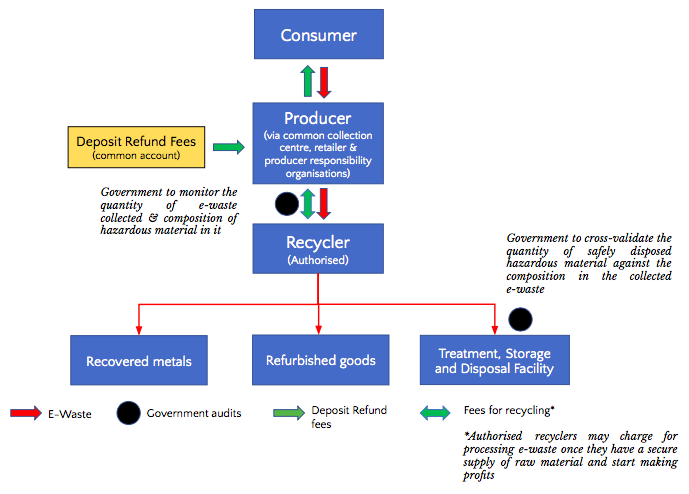
\includegraphics[height = 4.7in]{fig4.png}
\caption[Optional Caption]{The Revitalised EPR Model}
\end{figure}
                    
                    
%Possible Repercussions
\subsection{Possible Repercussions}
                    
                    The implementation of the proposed EPR model may also have certain unfavourable consequences. The changes in the demand for EEE would depend upon the price elasticity for particular goods. The Deposit fee could lead to an increase in smuggled devices, as the mandatory DRS would only be applicable in India and would raise the prices of domestic products. Each producer could also potentially lose consumers who will look for cheaper alternatives. 
                    
%Conclusion
\section*{Conclusion}
\addcontentsline{toc}{section}{Conclusion}
                    The quantity of e-waste generated in Delhi-NCR is projected to hit 1,50,000 MTA by 2020 \parencite{assochamdelhi}. Its potential for environmental and health hazards makes e-waste a critical issue to be dealt with.\\
                     
                     While the EPR model was a step in the right direction, it is yet to fulfil its aim. The informal sector processes over 95\% of e-waste in India, often handling it roughly without appropriate safety measures \parencite{assochamstats}. Moreover, it dumps the toxic residue without treating it properly.\\ 
                    
                    In this paper, we studied the current EPR model to account for its limitations and focused on the sharp difference in prices offered by the informal and authorised recyclers. Incentivised by these higher prices of the \textit{kabadiwala} or the local scrap dealer, consumers sold their products to the informal sector instead of returning the EEE to the producers.\\
                    
                    Our proposed modifications to the existing EPR model would tackle this price gap in three ways. The mandatory Deposit fee equalling or higher than the informal sector’s prices would keep the consumers from selling their products to the \textit{kabadiwala} and the Common Deposit Account would make it convenient for consumers to return their devices to the producers. Third-party audits would cross-check the amount of e-waste transferred from the producers with the quantity processed by the authorised recyclers. This would help ensure that the hazardous residue is treated properly.\\
                    
                    This is only a broad idea of how the EPR model can be reformed. Further research needs to be conducted to hammer out the execution. Aspects such as incentivising the reduction of hazardous substances in EEE and interest rate on the Deposit Refund fees have to be taken into account. Moreover, it is difficult to gather information on the different types of EEE and set the optimal quantum of fees that will direct e-waste to the authorised recyclers. Therefore, an alternate scenario where the market, instead of the government, can set the Deposit fee needs to be explored.

         
%Bibliography
\section*{Bibliography}
\addcontentsline{toc}{section}{Bibliography}
\printbibliography[heading=none] 
	     
	      
%Appendix 1
\newpage      
\section*{Appendix 1: Capacity of Recycling Firms}
\addcontentsline{toc}{section}{Appendix 1: Capacity of Recycling Firms }
         
\begin{table}[htpb]
\raggedright
\caption{Actual Working and Optimum Recycling Capacity of Surveyed Firms}\begin{tabular}{ l  c  c }
\toprule
\multicolumn{1}{p{7em}}{\raggedright{Name of Recycling Firm}} & \multicolumn{1}{p{8.5em}}{Optimum Capacity \centering\footnotesize\textit{(in tonnes)}} & \multicolumn{1}{p{9.5em}}{Capacity Utilised for 2017-18 \centering\footnotesize\textit{(in tonnes)}} \\
\midrule

Namo E-Waste Management, Faridabad & 5,796 & 870 \\
SMS Enterprises, Pace City, Gurgaon & 360 & 8 \\
Greeniva Recycler, Hapur & 1,500 & 700 \\
Royal Faiz Recycling, Hapur & 9,000 & 6,500 \\
Hind Recycling, Hapur & 9,000 & 2,000 \\
Earth Waste Management, Rohtak & 600 & 400 \\
\midrule
Total & 26,256 & 10,478  \\ 
\bottomrule
\end{tabular}
\end{table}
      
        
%Appendix 2
\section*{Appendix 2: Price Comparison Between Authorised and Informal Recyclers}
\addcontentsline{toc}{section}{Appendix 2: Price Comparison Between Authorised and Informal Recyclers}
       
\begin{table}[htpb]
\raggedright 
\caption{Price Comparison Between Authorised and Informal Recyclers}
\begin{tabular}{ l  r  r }
\toprule
 \multicolumn{1}{p{7em}}{\centering{Item}} & \multicolumn{1}{p{10em}}{Authorised Recyclers \raggedleft\footnotesize\textit{(Rs. per unit)}} & \multicolumn{1}{p{9.5em}}{\centering{Informal Recyclers} \raggedleft\footnotesize\textit{(Rs. per unit)}} \\
\midrule

HP Laptop (i3/i5) & 1,133.3 & 4,642.9\\
Refrigerator (350 litres) & 683.3 & 3,514.3 \\
Air Conditioner (AC) (1.5 tonnes) & 2,058.3 & 2,835.7 \\
HP CPU (500 GB 16 GB RAM) & 351.6  & 2,253.6 \\
LED TV (32-40 inches) & 436.6 & 2,107.1 \\
LCD TV (32-40 inches) & 403.3 & 1,642.9 \\
Samsung Mobile S6 & 62.5 & 1,418.6 \\
Printer (HP 1010) & 75.8 & 828.6 \\
Computer Monitor (15-17 inches) & 302.6 & 371.4\\
CRT TV (Colour) & 127.5 & 325 \\
UPS/Stabiliser & 112.5 & 324.3 \\
Toshiba Hard Disk (500 GB/1 TB) & 28.6 & 221.3 \\
Fax Machine & 40  & 197.9 \\ 
\bottomrule
\end{tabular}
\end{table}


%Appendix 3  
\newpage
\section*{Appendix 3: Additional Requirements for \\ Authorising Recyclers}
\addcontentsline{toc}{section}{Appendix 3: Additional Requirements for Authorising Recyclers}
        
        According to the Implementation Guidelines given by the CPCB for the EWM Rules, 2016, a recycling facility needs to provide the following to the SPCB:
            \begin{enumerate}[noitemsep,nolistsep]
            
                       \item Details of air pollution control devices along with a diagram and the design scheme
                        \item Details of effluent treatment plants (ETPs) installed in the unit along with a diagram and the design scheme 
                        \item Details of storage facility separate for raw material, segregated material, dismantled parts, hazardous waste, bag filter residue/floor cleaning dust, ETP sludge, non-recyclable/non-removable components
                             \item Membership and registration with a Treatment, Storage, Disposal Facility operator authorised under the HWM Rules, 2008
                              \item Power of attorney/authority letter of signature to the applicant
                               \item Details of handling, dismantling/recycling/refurbishing provided at the facility for e-waste and hazardous waste		                  
                               \begin{enumerate}[noitemsep,nolistsep]
                          	 	\item Should include adequate wastewater treatment facilities and air pollution control equipment 
                    	 		 \item Provide technology for data destruction 
                      		 \end{enumerate}
                       \item Copy of allotment letter from the Municipal Corporation with details of land and building plan \\
            \end{enumerate}
            
            Recyclers are also required to operate on a minimum of 500 sq. metres if their capacity is one metric tonne per day.\\
            
            The documents to be submitted for the Hazardous Waste (under the HWM Rules, 2016) Licence to the SPCB are:
        
        \begin{enumerate}[noitemsep,nolistsep]
        	\item Certificate authorising the Occupier (any person who has control over a factory that deals with hazardous and other wastes)
        	\item Nature and quantity of different wastes received annually from domestic sources or imports
        	\item Emergency Response Plan with procedures to be followed in an emergency such as a spillage or a fire
        	\item Details of the secured storage facility for hazardous wastes and their mode of disposal
        	\item Details of pollution control systems such as ETPs
        	\item Details of occupational health and safety measures
        	\item Process flow sheet showing equipment details, inputs (raw materials) and outputs (products, by-products, waste, emissions)
        	\item Details of the end user of products or by-products
        	\item Proof of application given to the operator of a Common Hazardous and Other Wastes Treatment, Storage and Disposal Facility (CHWTSDF)
        
        \end{enumerate}
        
      
         
         
%Appendix 4
\newpage       
\section*{Appendix 4: Questionnaire Administered to \\ Authorised Recyclers}
\addcontentsline{toc}{section}{Appendix 4: Questionnaire Administered to Authorised Recyclers}
\setstretch{0.5}
\begin{mdframed}[backgroundcolor=gray!20]

\begin{enumerate}[noitemsep,nolistsep]
                       \item General Information:
                          \begin{enumerate}[noitemsep]
                          	 \item Name of the firm
                    	  \item When was it established? (mm/yyyy)
                    	   \item Where is it located?
                       \end{enumerate}
                       \item When did you begin to acquire licences to register your firm? (mm/yyyy)
                       \item How long did it take to acquire all the licences necessary for registration?
                       \item Were you able to find clear guidelines for acquiring the licences on the SPCB website? 
                       \item Did you pay consultants/brokers/lawyers/others to help with the registration process? 
                       \item How long did it take for you to acquire the E-Waste Licence (under the EWM Rules, 2016)?
                       \item What were the official costs incurred to acquire the E-Waste Licence?
                       \item How long did it take for you to acquire the Hazardous Waste Licence (under the HWM Rules, 2016)? 
                        \item What were the official costs incurred to acquire the Hazardous Waste Licence? 
                        \item When did you start processing e-waste? (mm/yyyy) 
                        \item Who are your major sources of raw material?
                        \begin{enumerate}[noitemsep]
                          	 \item Local \textit{kabadiwalas}
                    	  \item Informal scrap dealers
                    	   \item Bulk consumers like IT companies 
                    	    \item Individual households 
                    	  \item Authorised Collectors/Producer Responsibility Organisations 
                    	   \item Others: \_\_\_\_
                       \end{enumerate}
                        \item What is the maximum recycling capacity of your firm? (in MTA)
                        \item What was the actual working capacity of your firm in the previous year? (in MTA)
                        \item What is the quantity of e-waste that is projected to be recycled by you in 2018? (in MTA) 
                         \item Has your firm reached its break-even point?
                         \item How long did it take to reach the break-even point after beginning operations? 
\end{enumerate}  
\end{mdframed}
                    
                                        
\end{document}